% ============================================================
\chapter{Root Finding}
\label{ch:roots}
% ============================================================

\section{Motivating example}
Finding $x$ such that $e^x = 3x$ amounts to finding a root of $f(x)=e^x-3x$. No closed-form solution exists: a numerical method is needed.

\section{Bisection method}

\begin{theorem}[Intermediate Value Theorem]\index{bisection}
If $f\in C([a,b])$ and $f(a)f(b)<0$, then $\exists\,c\in(a,b)$ such that $f(c)=0$.
\end{theorem}

\begin{algorithm}[H]
\caption{Bisection}\label{alg:bisection}
\KwInput{$f$, $a$, $b$, tolerance $\eps$}
\KwOutput{Approximation of the root $c$}
\While{$b-a > \eps$}{
  $c \gets (a+b)/2$\;
  \eIf{$f(a)\cdot f(c) < 0$}{$b \gets c$}{$a \gets c$}
}
\Return{$c$}
\end{algorithm}

\begin{theorem}[Convergence of bisection]
After $n$ iterations: $|c_n-x^*|\leq\frac{b-a}{2^{n+1}}$. The convergence is \textbf{linear} with rate $1/2$.
\end{theorem}

\begin{proof}
At each iteration, the interval is halved. After $n$ iterations, $|I_n|=(b-a)/2^n$ and $|c_n-x^*|\leq|I_n|/2$.
\end{proof}

\section{Newton's method}\index{Newton}

\begin{definition}
Newton's iteration for $f(x)=0$ is:
\[
x_{n+1} = x_n - \frac{f(x_n)}{f'(x_n)}.
\]
\end{definition}

\begin{center}
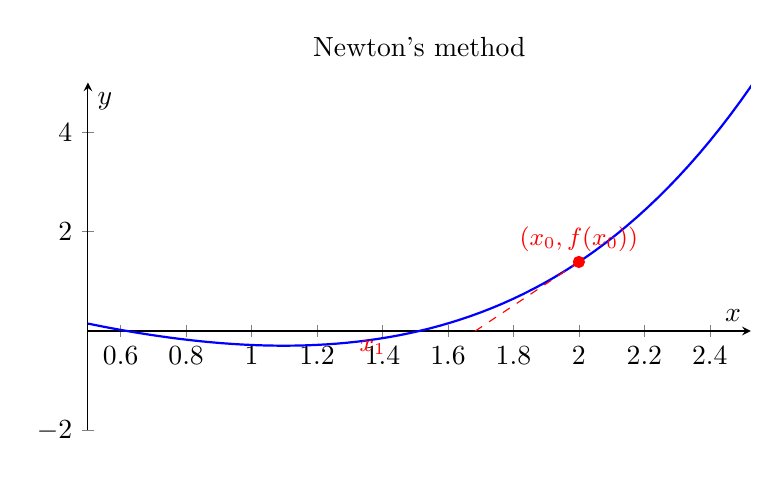
\begin{tikzpicture}
\begin{axis}[
  width=10cm, height=6cm, axis lines=middle,
  xlabel=$x$, ylabel=$y$, ymin=-2, ymax=5,
  domain=0.5:3, samples=80, title={Newton's method}
]
\addplot[thick,blue] {exp(x) - 3*x};
\addplot[dashed,red] coordinates {(2,{exp(2)-6}) (2-((exp(2)-6)/(exp(2)-3)),0)};
\addplot[only marks,mark=*,red] coordinates {(2,{exp(2)-6})};
\node[red,below] at (axis cs:1.37,0) {\small $x_1$};
\node[red,above] at (axis cs:2,1.4) {\small $(x_0,f(x_0))$};
\end{axis}
\end{tikzpicture}
\end{center}

\begin{algorithm}[H]
\caption{Newton's method}\label{alg:newton}
\KwInput{$f$, $f'$, $x_0$, tolerance $\eps$, $N_{\max}$}
\KwOutput{Approximation $x_n$}
\For{$n=0,1,\ldots,N_{\max}$}{
  $x_{n+1} \gets x_n - f(x_n)/f'(x_n)$\;
  \If{$|x_{n+1}-x_n|<\eps$}{\Return{$x_{n+1}$}}
}
\end{algorithm}

\begin{theorem}[Quadratic convergence of Newton's method]\label{thm:newton-conv}
If $f\in C^2$, $f(x^*)=0$, $f'(x^*)\neq 0$ and $x_0$ is sufficiently close to $x^*$, then:
\[
|e_{n+1}| \leq \frac{M}{2m}|e_n|^2,
\]
where $e_n=x_n-x^*$, $M=\sup|f''|$, $m=\inf|f'|$ in a neighbourhood of $x^*$.
\end{theorem}

\begin{proof}
By Taylor's theorem: $0=f(x^*)=f(x_n)+f'(x_n)(x^*-x_n)+\frac{f''(\xi_n)}{2}(x^*-x_n)^2$. Dividing by $f'(x_n)$:
\[
0 = \frac{f(x_n)}{f'(x_n)}+(x^*-x_n)+\frac{f''(\xi_n)}{2f'(x_n)}e_n^2.
\]
Since $x_{n+1}=x_n-f(x_n)/f'(x_n)$, we get $e_{n+1}=x_{n+1}-x^*=-\frac{f''(\xi_n)}{2f'(x_n)}e_n^2$.
\end{proof}

\section{Secant method}\index{secant method}

\begin{definition}
We replace $f'(x_n)$ by a finite difference:
\[
x_{n+1} = x_n - f(x_n)\frac{x_n-x_{n-1}}{f(x_n)-f(x_{n-1})}.
\]
\end{definition}

\begin{theorem}
The order of convergence of the secant method is the \textbf{golden ratio} $\varphi=(1+\sqrt{5})/2\approx 1.618$.
\end{theorem}

\section{Fixed-point method}\index{fixed point}

\begin{definition}
Find $x=g(x)$. Iteration: $x_{n+1}=g(x_n)$.
\end{definition}

\begin{theorem}[Banach Fixed-Point Theorem]\label{thm:banach}
If $g:[a,b]\to[a,b]$ is a contraction ($|g'(x)|\leq L<1$ on $[a,b]$), then $g$ has a unique fixed point $x^*$ and $x_n\to x^*$ with:
\[
|x_n-x^*|\leq \frac{L^n}{1-L}|x_1-x_0|.
\]
\end{theorem}

\section{Comparison of methods}

\begin{center}
\begin{tabular}{lccc}
\toprule
\textbf{Method} & \textbf{Order} & \textbf{Evaluations of $f$} & \textbf{Robustness} \\
\midrule
Bisection & 1 (linear) & 1/iter. & Very robust \\
Newton & 2 (quadratic) & $f + f'$/iter. & Sensitive to $x_0$ \\
Secant & $\varphi\approx 1.618$ & 1/iter. & Moderate \\
\bottomrule
\end{tabular}
\end{center}

\section{Numerical example}

Root of $f(x)=e^x-3x$ with $x_0=2$ (Newton):
\begin{center}
\begin{tabular}{cccc}
\toprule
$n$ & $x_n$ & $f(x_n)$ & $|x_n-x_{n-1}|$ \\
\midrule
0 & 2.000000 & 1.389056 & --- \\
1 & 1.373418 & 0.225698 & 0.627 \\
2 & 1.524247 & $-0.046$ & 0.151 \\
3 & 1.512127 & $-0.000374$ & 0.012 \\
4 & 1.512135 & $<10^{-9}$ & $8\times10^{-6}$ \\
\bottomrule
\end{tabular}
\end{center}

\section{Implementation}

\begin{codeblock}[title=\textbf{Python}]
\begin{minted}{python}
import numpy as np

def bisection(f, a, b, tol=1e-12):
    while b - a > tol:
        c = (a + b) / 2
        if f(a) * f(c) < 0:
            b = c
        else:
            a = c
    return (a + b) / 2

def newton(f, df, x0, tol=1e-12, maxiter=100):
    x = x0
    for i in range(maxiter):
        dx = f(x) / df(x)
        x -= dx
        if abs(dx) < tol:
            return x, i+1
    return x, maxiter

def secant(f, x0, x1, tol=1e-12, maxiter=100):
    for i in range(maxiter):
        fx0, fx1 = f(x0), f(x1)
        x2 = x1 - fx1 * (x1 - x0) / (fx1 - fx0)
        if abs(x2 - x1) < tol:
            return x2, i+1
        x0, x1 = x1, x2
    return x1, maxiter

# Test
f = lambda x: np.exp(x) - 3*x
df = lambda x: np.exp(x) - 3

print(f"Bissection : {bisection(f, 0, 1):.12f}")
x_newton, n = newton(f, df, 2.0)
print(f"Newton     : {x_newton:.12f} ({n} iterations)")
x_sec, n = secant(f, 0.0, 1.0)
print(f"Secante    : {x_sec:.12f} ({n} iterations)")
\end{minted}
\end{codeblock}

\begin{codeblock}[title=\textbf{Julia}]
\begin{minted}{julia}
function newton(f, df, x0; tol=1e-12, maxiter=100)
    x = x0
    for i in 1:maxiter
        dx = f(x) / df(x)
        x -= dx
        abs(dx) < tol && return x, i
    end
    return x, maxiter
end

f(x) = exp(x) - 3x
df(x) = exp(x) - 3
x, n = newton(f, df, 2.0)
println("Newton: x = $x ($n iterations)")
\end{minted}
\end{codeblock}

\section{Exercises}

\begin{exercise}[$\star$]
Find $\sqrt{2}$ by applying Newton's method to $f(x)=x^2-2$. How many iterations are needed for 15 decimal digits?
\end{exercise}

\begin{exercise}[$\star\star$]
Show that Newton's method applied to $f(x)=x^2$ converges linearly (double root). Generalise: what happens when $f'(x^*)=0$?
\end{exercise}

\begin{exercise}[$\star\star$]
Prove that the order of the secant method is $\varphi$ by setting $e_{n+1}\approx C\,e_n^p$ and solving $p^2-p-1=0$.
\end{exercise}

\begin{exercise}[$\star\star\star$ -- Project]
Implement Brent's method (combination of bisection + secant). Compare with the simpler methods on 10 test functions.
\end{exercise}

\begin{keyformulas}
\begin{align*}
\text{Bisection} &: |e_n|\leq\frac{b-a}{2^{n+1}} \\
\text{Newton} &: x_{n+1}=x_n-\frac{f(x_n)}{f'(x_n)},\quad |e_{n+1}|\leq C|e_n|^2 \\
\text{Secant} &: x_{n+1}=x_n-f(x_n)\frac{x_n-x_{n-1}}{f(x_n)-f(x_{n-1})},\quad \text{order }\varphi
\end{align*}
\end{keyformulas}
